% Options for packages loaded elsewhere
\PassOptionsToPackage{unicode}{hyperref}
\PassOptionsToPackage{hyphens}{url}
%
\documentclass[
]{article}
\usepackage{lmodern}
\usepackage{amssymb,amsmath}
\usepackage{ifxetex,ifluatex}
\ifnum 0\ifxetex 1\fi\ifluatex 1\fi=0 % if pdftex
  \usepackage[T1]{fontenc}
  \usepackage[utf8]{inputenc}
  \usepackage{textcomp} % provide euro and other symbols
\else % if luatex or xetex
  \usepackage{unicode-math}
  \defaultfontfeatures{Scale=MatchLowercase}
  \defaultfontfeatures[\rmfamily]{Ligatures=TeX,Scale=1}
\fi
% Use upquote if available, for straight quotes in verbatim environments
\IfFileExists{upquote.sty}{\usepackage{upquote}}{}
\IfFileExists{microtype.sty}{% use microtype if available
  \usepackage[]{microtype}
  \UseMicrotypeSet[protrusion]{basicmath} % disable protrusion for tt fonts
}{}
\makeatletter
\@ifundefined{KOMAClassName}{% if non-KOMA class
  \IfFileExists{parskip.sty}{%
    \usepackage{parskip}
  }{% else
    \setlength{\parindent}{0pt}
    \setlength{\parskip}{6pt plus 2pt minus 1pt}}
}{% if KOMA class
  \KOMAoptions{parskip=half}}
\makeatother
\usepackage{xcolor}
\IfFileExists{xurl.sty}{\usepackage{xurl}}{} % add URL line breaks if available
\IfFileExists{bookmark.sty}{\usepackage{bookmark}}{\usepackage{hyperref}}
\hypersetup{
  pdftitle={Simple 3-state Markov model in R},
  pdfauthor={The DARTH workgroup},
  hidelinks,
  pdfcreator={LaTeX via pandoc}}
\urlstyle{same} % disable monospaced font for URLs
\usepackage[margin=1in]{geometry}
\usepackage{color}
\usepackage{fancyvrb}
\newcommand{\VerbBar}{|}
\newcommand{\VERB}{\Verb[commandchars=\\\{\}]}
\DefineVerbatimEnvironment{Highlighting}{Verbatim}{commandchars=\\\{\}}
% Add ',fontsize=\small' for more characters per line
\usepackage{framed}
\definecolor{shadecolor}{RGB}{248,248,248}
\newenvironment{Shaded}{\begin{snugshade}}{\end{snugshade}}
\newcommand{\AlertTok}[1]{\textcolor[rgb]{0.94,0.16,0.16}{#1}}
\newcommand{\AnnotationTok}[1]{\textcolor[rgb]{0.56,0.35,0.01}{\textbf{\textit{#1}}}}
\newcommand{\AttributeTok}[1]{\textcolor[rgb]{0.77,0.63,0.00}{#1}}
\newcommand{\BaseNTok}[1]{\textcolor[rgb]{0.00,0.00,0.81}{#1}}
\newcommand{\BuiltInTok}[1]{#1}
\newcommand{\CharTok}[1]{\textcolor[rgb]{0.31,0.60,0.02}{#1}}
\newcommand{\CommentTok}[1]{\textcolor[rgb]{0.56,0.35,0.01}{\textit{#1}}}
\newcommand{\CommentVarTok}[1]{\textcolor[rgb]{0.56,0.35,0.01}{\textbf{\textit{#1}}}}
\newcommand{\ConstantTok}[1]{\textcolor[rgb]{0.00,0.00,0.00}{#1}}
\newcommand{\ControlFlowTok}[1]{\textcolor[rgb]{0.13,0.29,0.53}{\textbf{#1}}}
\newcommand{\DataTypeTok}[1]{\textcolor[rgb]{0.13,0.29,0.53}{#1}}
\newcommand{\DecValTok}[1]{\textcolor[rgb]{0.00,0.00,0.81}{#1}}
\newcommand{\DocumentationTok}[1]{\textcolor[rgb]{0.56,0.35,0.01}{\textbf{\textit{#1}}}}
\newcommand{\ErrorTok}[1]{\textcolor[rgb]{0.64,0.00,0.00}{\textbf{#1}}}
\newcommand{\ExtensionTok}[1]{#1}
\newcommand{\FloatTok}[1]{\textcolor[rgb]{0.00,0.00,0.81}{#1}}
\newcommand{\FunctionTok}[1]{\textcolor[rgb]{0.00,0.00,0.00}{#1}}
\newcommand{\ImportTok}[1]{#1}
\newcommand{\InformationTok}[1]{\textcolor[rgb]{0.56,0.35,0.01}{\textbf{\textit{#1}}}}
\newcommand{\KeywordTok}[1]{\textcolor[rgb]{0.13,0.29,0.53}{\textbf{#1}}}
\newcommand{\NormalTok}[1]{#1}
\newcommand{\OperatorTok}[1]{\textcolor[rgb]{0.81,0.36,0.00}{\textbf{#1}}}
\newcommand{\OtherTok}[1]{\textcolor[rgb]{0.56,0.35,0.01}{#1}}
\newcommand{\PreprocessorTok}[1]{\textcolor[rgb]{0.56,0.35,0.01}{\textit{#1}}}
\newcommand{\RegionMarkerTok}[1]{#1}
\newcommand{\SpecialCharTok}[1]{\textcolor[rgb]{0.00,0.00,0.00}{#1}}
\newcommand{\SpecialStringTok}[1]{\textcolor[rgb]{0.31,0.60,0.02}{#1}}
\newcommand{\StringTok}[1]{\textcolor[rgb]{0.31,0.60,0.02}{#1}}
\newcommand{\VariableTok}[1]{\textcolor[rgb]{0.00,0.00,0.00}{#1}}
\newcommand{\VerbatimStringTok}[1]{\textcolor[rgb]{0.31,0.60,0.02}{#1}}
\newcommand{\WarningTok}[1]{\textcolor[rgb]{0.56,0.35,0.01}{\textbf{\textit{#1}}}}
\usepackage{graphicx,grffile}
\makeatletter
\def\maxwidth{\ifdim\Gin@nat@width>\linewidth\linewidth\else\Gin@nat@width\fi}
\def\maxheight{\ifdim\Gin@nat@height>\textheight\textheight\else\Gin@nat@height\fi}
\makeatother
% Scale images if necessary, so that they will not overflow the page
% margins by default, and it is still possible to overwrite the defaults
% using explicit options in \includegraphics[width, height, ...]{}
\setkeys{Gin}{width=\maxwidth,height=\maxheight,keepaspectratio}
% Set default figure placement to htbp
\makeatletter
\def\fps@figure{htbp}
\makeatother
\setlength{\emergencystretch}{3em} % prevent overfull lines
\providecommand{\tightlist}{%
  \setlength{\itemsep}{0pt}\setlength{\parskip}{0pt}}
\setcounter{secnumdepth}{-\maxdimen} % remove section numbering

\title{Simple 3-state Markov model in R}
\author{The DARTH workgroup}
\date{}

\begin{document}
\maketitle

Developed by the Decision Analysis in R for Technologies in Health
(DARTH) workgroup:

Fernando Alarid-Escudero, PhD (1)

Eva A. Enns, MS, PhD (2)

M.G. Myriam Hunink, MD, PhD (3,4)

Hawre J. Jalal, MD, PhD (5)

Eline M. Krijkamp, MSc (3)

Petros Pechlivanoglou, PhD (6,7)

Alan Yang, MSc (7)

In collaboration of:

\begin{enumerate}
\def\labelenumi{\arabic{enumi}.}
\tightlist
\item
  Drug Policy Program, Center for Research and Teaching in Economics
  (CIDE) - CONACyT, Aguascalientes, Mexico
\item
  University of Minnesota School of Public Health, Minneapolis, MN, USA
\item
  Erasmus MC, Rotterdam, The Netherlands
\item
  Harvard T.H. Chan School of Public Health, Boston, USA
\item
  University of Pittsburgh Graduate School of Public Health, Pittsburgh,
  PA, USA
\item
  University of Toronto, Toronto ON, Canada
\item
  The Hospital for Sick Children, Toronto ON, Canada
\end{enumerate}

Please cite our publications when using this code:

\begin{itemize}
\item
  Jalal H, Pechlivanoglou P, Krijkamp E, Alarid-Escudero F, Enns E,
  Hunink MG. An Overview of R in Health Decision Sciences. Med Decis
  Making. 2017; 37(3): 735-746.
  \url{https://journals.sagepub.com/doi/abs/10.1177/0272989X16686559}
\item
  Krijkamp EM, Alarid-Escudero F, Enns EA, Jalal HJ, Hunink MGM,
  Pechlivanoglou P. Microsimulation modeling for health decision
  sciences using R: A tutorial. Med Decis Making. 2018;38(3):400--22.
  \url{https://journals.sagepub.com/doi/abs/10.1177/0272989X18754513}
\item
  Krijkamp EM, Alarid-Escudero F, Enns E, Pechlivanoglou P, Hunink MM,
  Jalal H. A Multidimensional Array Representation of State-Transition
  Model Dynamics. Med Decis Making. Online First
  \url{https://doi.org/10.1177/0272989X19893973}
\end{itemize}

Copyright 2017, THE HOSPITAL FOR SICK CHILDREN AND THE COLLABORATING
INSTITUTIONS. All rights reserved in Canada, the United States and
worldwide. Copyright, trademarks, trade names and any and all associated
intellectual property are exclusively owned by THE HOSPITAL FOR Sick
CHILDREN and the collaborating institutions. These materials may be
used, reproduced, modified, distributed and adapted with proper
attribution.

\newpage

\begin{Shaded}
\begin{Highlighting}[]
\KeywordTok{rm}\NormalTok{(}\DataTypeTok{list =} \KeywordTok{ls}\NormalTok{())      }\CommentTok{# clear memory (removes all the variables from the workspace)}
\end{Highlighting}
\end{Shaded}

\hypertarget{load-packages}{%
\section{01 Load packages}\label{load-packages}}

\begin{Shaded}
\begin{Highlighting}[]
\ControlFlowTok{if}\NormalTok{ (}\OperatorTok{!}\KeywordTok{require}\NormalTok{(}\StringTok{'pacman'}\NormalTok{)) }\KeywordTok{install.packages}\NormalTok{(}\StringTok{'pacman'}\NormalTok{); }\KeywordTok{library}\NormalTok{(pacman) }\CommentTok{# use this package to conveniently install other packages}
\end{Highlighting}
\end{Shaded}

\begin{verbatim}
## Loading required package: pacman
\end{verbatim}

\begin{Shaded}
\begin{Highlighting}[]
\CommentTok{# load (install if required) packages from CRAN}
\KeywordTok{p_load}\NormalTok{(}\StringTok{"diagram"}\NormalTok{) }
\end{Highlighting}
\end{Shaded}

\hypertarget{load-functions}{%
\section{02 Load functions}\label{load-functions}}

\begin{Shaded}
\begin{Highlighting}[]
\CommentTok{# no functions required}
\end{Highlighting}
\end{Shaded}

\hypertarget{input-model-parameters}{%
\section{03 Input model parameters}\label{input-model-parameters}}

\begin{Shaded}
\begin{Highlighting}[]
\CommentTok{# Strategy names}
\NormalTok{v_names_str <-}\StringTok{ }\KeywordTok{c}\NormalTok{(}\StringTok{"Base Case"}\NormalTok{)  }

\CommentTok{# Number of strategies}
\NormalTok{n_str <-}\StringTok{ }\KeywordTok{length}\NormalTok{(v_names_str)}

\CommentTok{# Markov model parameters}
\NormalTok{v_n  <-}\StringTok{ }\KeywordTok{c}\NormalTok{(}\StringTok{"Healthy"}\NormalTok{, }\StringTok{"Sick"}\NormalTok{, }\StringTok{"Dead"}\NormalTok{)    }\CommentTok{# state names}
\NormalTok{n_states  <-}\StringTok{ }\KeywordTok{length}\NormalTok{(v_n)                }\CommentTok{# number of states}
\NormalTok{n_t  <-}\StringTok{ }\DecValTok{60}                              \CommentTok{# number of cycles}

\NormalTok{p_HD <-}\StringTok{ }\FloatTok{0.02}                            \CommentTok{# probability to die when healthy}
\NormalTok{p_HS <-}\StringTok{ }\FloatTok{0.05}                            \CommentTok{# probability to become sick when healthy}
\NormalTok{p_SD <-}\StringTok{ }\FloatTok{0.1}                             \CommentTok{# probability to die when sick}

\CommentTok{# Costs and utilities  }
\NormalTok{c_H  <-}\StringTok{ }\DecValTok{400}                             \CommentTok{# cost of remaining one cycle healthy}
\NormalTok{c_S  <-}\StringTok{ }\DecValTok{1000}                            \CommentTok{# cost of remaining one cycle sick}
\NormalTok{c_D  <-}\StringTok{ }\DecValTok{0}                               \CommentTok{# cost of remaining one cycle dead}
\NormalTok{u_H  <-}\StringTok{ }\FloatTok{0.8}                             \CommentTok{# utility when healthy }
\NormalTok{u_S  <-}\StringTok{ }\FloatTok{0.5}                             \CommentTok{# utility when sick}
\NormalTok{u_D  <-}\StringTok{ }\DecValTok{0}                               \CommentTok{# utility when dead}
\NormalTok{d_e  <-}\StringTok{ }\NormalTok{d_c <-}\StringTok{ }\FloatTok{0.03}                     \CommentTok{# equal discount of costs and QALYs by 3%}

\CommentTok{# calculate discount weights for costs for each cycle based on discount rate d_c}
\NormalTok{v_dwc <-}\StringTok{ }\DecValTok{1} \OperatorTok{/}\StringTok{ }\NormalTok{(}\DecValTok{1} \OperatorTok{+}\StringTok{ }\NormalTok{d_e) }\OperatorTok{^}\StringTok{ }\NormalTok{(}\DecValTok{0}\OperatorTok{:}\NormalTok{n_t) }
\CommentTok{# calculate discount weights for effectiveness for each cycle based on discount rate d_e}
\NormalTok{v_dwe <-}\StringTok{ }\DecValTok{1} \OperatorTok{/}\StringTok{ }\NormalTok{(}\DecValTok{1} \OperatorTok{+}\StringTok{ }\NormalTok{d_c) }\OperatorTok{^}\StringTok{ }\NormalTok{(}\DecValTok{0}\OperatorTok{:}\NormalTok{n_t) }
\end{Highlighting}
\end{Shaded}

\hypertarget{draw-the-state-transition-cohort-model}{%
\subsection{Draw the state-transition cohort
model}\label{draw-the-state-transition-cohort-model}}

\begin{Shaded}
\begin{Highlighting}[]
\NormalTok{m_P_diag <-}\StringTok{ }\KeywordTok{matrix}\NormalTok{(}\DecValTok{0}\NormalTok{, }\DataTypeTok{nrow =}\NormalTok{ n_states, }\DataTypeTok{ncol =}\NormalTok{ n_states, }\DataTypeTok{dimnames =} \KeywordTok{list}\NormalTok{(v_n, v_n))}
\NormalTok{m_P_diag[}\StringTok{"Healthy"}\NormalTok{, }\StringTok{"Sick"}\NormalTok{ ]     =}\StringTok{ ""} 
\NormalTok{m_P_diag[}\StringTok{"Healthy"}\NormalTok{, }\StringTok{"Dead"}\NormalTok{ ]     =}\StringTok{ ""}
\NormalTok{m_P_diag[}\StringTok{"Healthy"}\NormalTok{, }\StringTok{"Healthy"}\NormalTok{ ]  =}\StringTok{ ""}
\NormalTok{m_P_diag[}\StringTok{"Sick"}\NormalTok{   , }\StringTok{"Dead"}\NormalTok{ ]     =}\StringTok{ ""}
\NormalTok{m_P_diag[}\StringTok{"Sick"}\NormalTok{   , }\StringTok{"Sick"}\NormalTok{ ]     =}\StringTok{ ""}
\NormalTok{m_P_diag[}\StringTok{"Dead"}\NormalTok{   , }\StringTok{"Dead"}\NormalTok{ ]     =}\StringTok{ ""}
\NormalTok{layout.fig <-}\StringTok{ }\KeywordTok{c}\NormalTok{(}\DecValTok{2}\NormalTok{, }\DecValTok{1}\NormalTok{)}
\KeywordTok{plotmat}\NormalTok{(}\KeywordTok{t}\NormalTok{(m_P_diag), }\KeywordTok{t}\NormalTok{(layout.fig), }\DataTypeTok{self.cex =} \FloatTok{0.5}\NormalTok{, }\DataTypeTok{curve =} \DecValTok{0}\NormalTok{, }\DataTypeTok{arr.pos =} \FloatTok{0.8}\NormalTok{,  }
        \DataTypeTok{latex =}\NormalTok{ T, }\DataTypeTok{arr.type =} \StringTok{"curved"}\NormalTok{, }\DataTypeTok{relsize =} \FloatTok{0.85}\NormalTok{, }\DataTypeTok{box.prop =} \FloatTok{0.8}\NormalTok{, }
        \DataTypeTok{cex =} \FloatTok{0.8}\NormalTok{, }\DataTypeTok{box.cex =} \FloatTok{0.7}\NormalTok{, }\DataTypeTok{lwd =} \DecValTok{1}\NormalTok{)}
\end{Highlighting}
\end{Shaded}

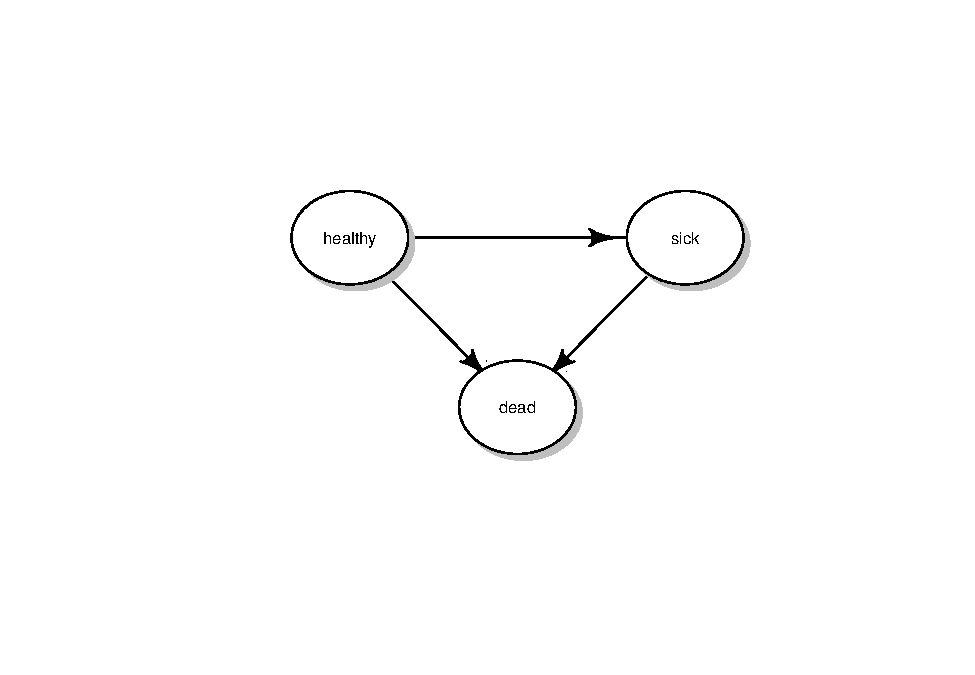
\includegraphics{Markov_3state_files/figure-latex/unnamed-chunk-5-1.pdf}

\hypertarget{define-and-initialize-matrices-and-vectors}{%
\section{04 Define and initialize matrices and
vectors}\label{define-and-initialize-matrices-and-vectors}}

\hypertarget{cohort-trace}{%
\subsection{04.1 Cohort trace}\label{cohort-trace}}

\begin{Shaded}
\begin{Highlighting}[]
\CommentTok{# create the cohort trace}
\NormalTok{m_M <-}\StringTok{ }\KeywordTok{matrix}\NormalTok{(}\OtherTok{NA}\NormalTok{, }
              \DataTypeTok{nrow =}\NormalTok{ n_t }\OperatorTok{+}\StringTok{ }\DecValTok{1}\NormalTok{ ,  }\CommentTok{# create Markov trace (n.t + 1 because R doesn't }
                                \CommentTok{# understand Cycle 0)}
              \DataTypeTok{ncol =}\NormalTok{ n_states, }
              \DataTypeTok{dimnames =} \KeywordTok{list}\NormalTok{(}\DecValTok{0}\OperatorTok{:}\NormalTok{n_t, v_n))}

\NormalTok{m_M[}\DecValTok{1}\NormalTok{, ] <-}\StringTok{ }\KeywordTok{c}\NormalTok{(}\DecValTok{1}\NormalTok{, }\DecValTok{0}\NormalTok{, }\DecValTok{0}\NormalTok{)          }\CommentTok{# initialize first cycle of Markov trace}
\end{Highlighting}
\end{Shaded}

\hypertarget{transition-probability-matrix}{%
\subsection{04.2 Transition probability
matrix}\label{transition-probability-matrix}}

\begin{Shaded}
\begin{Highlighting}[]
\CommentTok{# create the transition probability matrix}
\NormalTok{m_P  <-}\StringTok{ }\KeywordTok{matrix}\NormalTok{(}\DecValTok{0}\NormalTok{,}
               \DataTypeTok{nrow =}\NormalTok{ n_states, }\DataTypeTok{ncol =}\NormalTok{ n_states,}
               \DataTypeTok{dimnames =} \KeywordTok{list}\NormalTok{(v_n, v_n)) }\CommentTok{# name the columns and rows of the transition }
                                          \CommentTok{# probability matrix}
\NormalTok{m_P}
\end{Highlighting}
\end{Shaded}

\begin{verbatim}
##         Healthy Sick Dead
## Healthy       0    0    0
## Sick          0    0    0
## Dead          0    0    0
\end{verbatim}

Fill in the transition probability matrix:

\begin{Shaded}
\begin{Highlighting}[]
\CommentTok{# from Healthy}
\NormalTok{m_P[}\StringTok{"Healthy"}\NormalTok{, }\StringTok{"Healthy"}\NormalTok{] <-}\StringTok{ }\DecValTok{1} \OperatorTok{-}\StringTok{ }\NormalTok{p_HD }\OperatorTok{-}\StringTok{ }\NormalTok{p_HS}
\NormalTok{m_P[}\StringTok{"Healthy"}\NormalTok{, }\StringTok{"Sick"}\NormalTok{]    <-}\StringTok{ }\NormalTok{p_HS}
\NormalTok{m_P[}\StringTok{"Healthy"}\NormalTok{, }\StringTok{"Dead"}\NormalTok{]    <-}\StringTok{ }\NormalTok{p_HD}

\CommentTok{# from Sick}
\NormalTok{m_P[}\StringTok{"Sick"}\NormalTok{, }\StringTok{"Sick"}\NormalTok{] <-}\StringTok{ }\DecValTok{1} \OperatorTok{-}\StringTok{ }\NormalTok{p_SD}
\NormalTok{m_P[}\StringTok{"Sick"}\NormalTok{, }\StringTok{"Dead"}\NormalTok{] <-}\StringTok{ }\NormalTok{p_SD}

\CommentTok{# from Dead}
\NormalTok{m_P[}\StringTok{"Dead"}\NormalTok{, }\StringTok{"Dead"}\NormalTok{] <-}\StringTok{ }\DecValTok{1}

\CommentTok{# check rows add up to 1}
\KeywordTok{rowSums}\NormalTok{(m_P)}
\end{Highlighting}
\end{Shaded}

\begin{verbatim}
## Healthy    Sick    Dead 
##       1       1       1
\end{verbatim}

\hypertarget{run-markov-model}{%
\section{05 Run Markov model}\label{run-markov-model}}

\begin{Shaded}
\begin{Highlighting}[]
\ControlFlowTok{for}\NormalTok{ (t }\ControlFlowTok{in} \DecValTok{1}\OperatorTok{:}\NormalTok{n_t)\{                   }\CommentTok{# loop through the number of cycles}
\NormalTok{  m_M[t }\OperatorTok{+}\StringTok{ }\DecValTok{1}\NormalTok{, ] <-}\StringTok{ }\NormalTok{m_M[t, ] }\OperatorTok\StringTok{ }\NormalTok{m_P  }\CommentTok{# estimate the state vector for the next cycle (t + 1)}
\NormalTok{\}}
\end{Highlighting}
\end{Shaded}

\hypertarget{compute-and-plot-epidemiological-outcomes}{%
\section{06 Compute and Plot Epidemiological
Outcomes}\label{compute-and-plot-epidemiological-outcomes}}

\hypertarget{cohort-trace-1}{%
\subsection{06.1 Cohort trace}\label{cohort-trace-1}}

\begin{Shaded}
\begin{Highlighting}[]
\KeywordTok{matplot}\NormalTok{(m_M, }\DataTypeTok{type =} \StringTok{'l'}\NormalTok{, }
        \DataTypeTok{ylab =} \StringTok{"Probability of state occupancy"}\NormalTok{,}
        \DataTypeTok{xlab =} \StringTok{"Cycle"}\NormalTok{,}
        \DataTypeTok{main =} \StringTok{"Cohort Trace"}\NormalTok{, }\DataTypeTok{lwd =} \DecValTok{3}\NormalTok{)                 }\CommentTok{# create a plot of the data}
\KeywordTok{legend}\NormalTok{(}\StringTok{"right"}\NormalTok{, v_n, }\DataTypeTok{col =} \KeywordTok{c}\NormalTok{(}\StringTok{"black"}\NormalTok{, }\StringTok{"red"}\NormalTok{, }\StringTok{"green"}\NormalTok{), }
       \DataTypeTok{lty =} \DecValTok{1}\OperatorTok{:}\DecValTok{3}\NormalTok{, }\DataTypeTok{bty =} \StringTok{"n"}\NormalTok{)                            }\CommentTok{# add a legend to the graph}

\KeywordTok{abline}\NormalTok{(}\DataTypeTok{v =} \KeywordTok{which.max}\NormalTok{(m_M[, }\StringTok{"Sick"}\NormalTok{]), }\DataTypeTok{col =} \StringTok{"gray"}\NormalTok{) }\CommentTok{# plot a vertical line that helps identifying at which cycle the prevalence of sick is highest.  }
\end{Highlighting}
\end{Shaded}

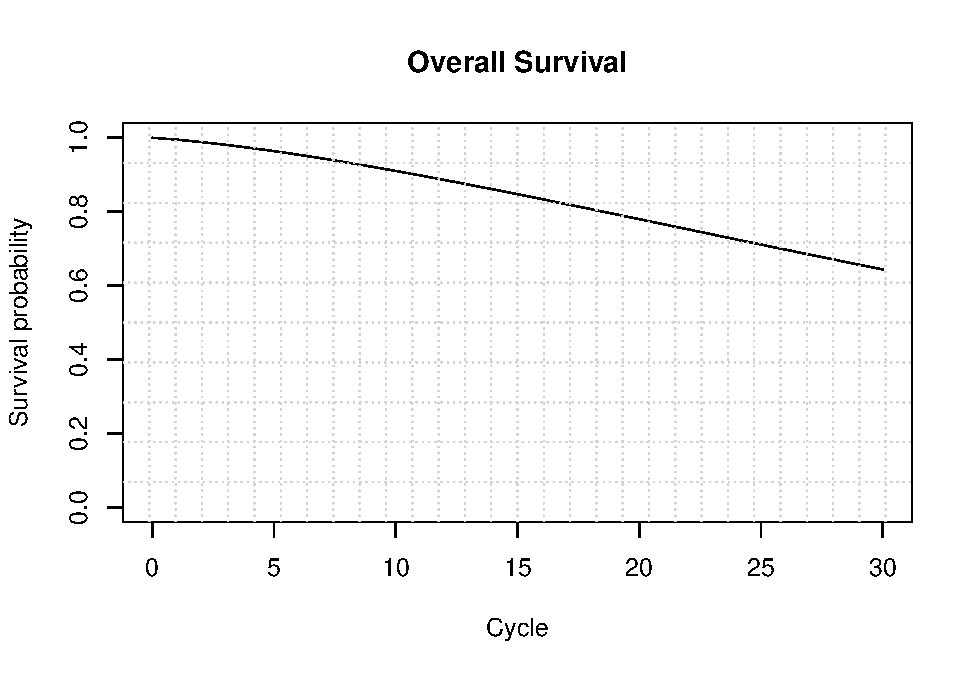
\includegraphics{Markov_3state_files/figure-latex/unnamed-chunk-10-1.pdf}

\hypertarget{overall-survival-os}{%
\subsection{06.2 Overall Survival (OS)}\label{overall-survival-os}}

\begin{Shaded}
\begin{Highlighting}[]
\NormalTok{v_os <-}\StringTok{ }\DecValTok{1} \OperatorTok{-}\StringTok{ }\NormalTok{m_M[, }\StringTok{"Dead"}\NormalTok{]             }\CommentTok{# calculate the overall survival (OS) probability}
\NormalTok{v_os <-}\StringTok{ }\KeywordTok{rowSums}\NormalTok{(m_M[, }\DecValTok{1}\OperatorTok{:}\DecValTok{2}\NormalTok{])           }\CommentTok{# alternative way of calculating the OS probability   }

\KeywordTok{plot}\NormalTok{(v_os, }\DataTypeTok{type =} \StringTok{'l'}\NormalTok{, }
     \DataTypeTok{ylim =} \KeywordTok{c}\NormalTok{(}\DecValTok{0}\NormalTok{, }\DecValTok{1}\NormalTok{),}
     \DataTypeTok{ylab =} \StringTok{"Survival probability"}\NormalTok{,}
     \DataTypeTok{xlab =} \StringTok{"Cycle"}\NormalTok{,}
     \DataTypeTok{main =} \StringTok{"Overall Survival"}\NormalTok{)       }\CommentTok{# create a simple plot showing the OS}

\CommentTok{# add grid }
\KeywordTok{grid}\NormalTok{(}\DataTypeTok{nx =}\NormalTok{ n_t, }\DataTypeTok{ny =} \DecValTok{10}\NormalTok{, }\DataTypeTok{col =} \StringTok{"lightgray"}\NormalTok{, }\DataTypeTok{lty =} \StringTok{"dotted"}\NormalTok{, }\DataTypeTok{lwd =} \KeywordTok{par}\NormalTok{(}\StringTok{"lwd"}\NormalTok{), }
     \DataTypeTok{equilogs =} \OtherTok{TRUE}\NormalTok{) }
\end{Highlighting}
\end{Shaded}

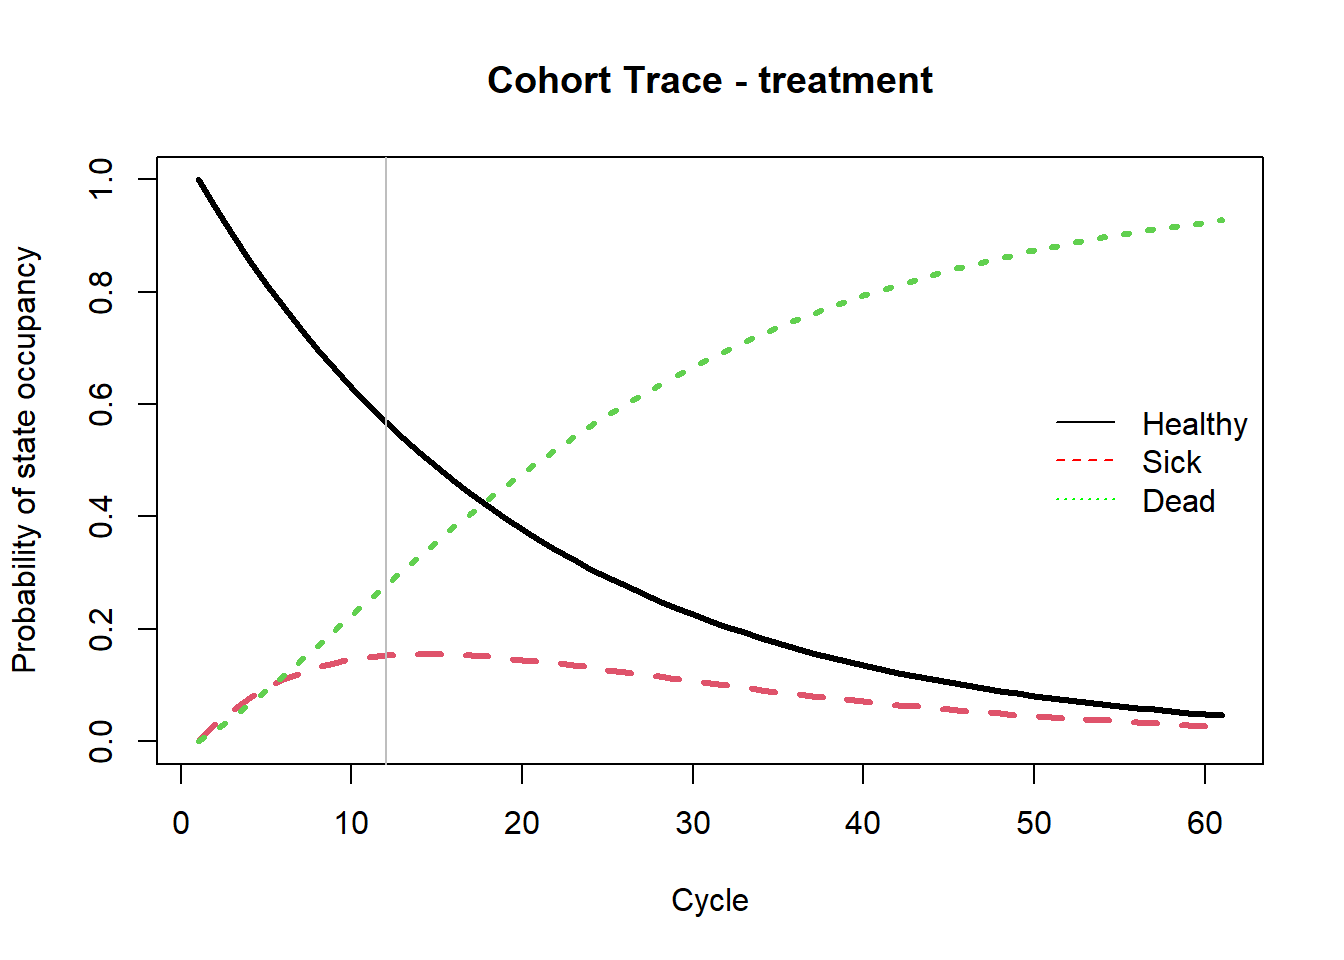
\includegraphics{Markov_3state_files/figure-latex/unnamed-chunk-11-1.pdf}

\hypertarget{life-expectancy-le}{%
\subsection{06.2.1 Life Expectancy (LE)}\label{life-expectancy-le}}

\begin{Shaded}
\begin{Highlighting}[]
\NormalTok{v_le <-}\StringTok{ }\KeywordTok{sum}\NormalTok{(v_os)           }\CommentTok{# summing probablity of OS over time  (i.e. life expectancy)}
\end{Highlighting}
\end{Shaded}

\hypertarget{disease-prevalence}{%
\subsection{06.3 Disease prevalence}\label{disease-prevalence}}

\begin{Shaded}
\begin{Highlighting}[]
\NormalTok{v_prev <-}\StringTok{ }\NormalTok{m_M[, }\StringTok{"Sick"}\NormalTok{]}\OperatorTok{/}\NormalTok{v_os}
\KeywordTok{plot}\NormalTok{(v_prev,}
     \DataTypeTok{ylim =} \KeywordTok{c}\NormalTok{(}\DecValTok{0}\NormalTok{, }\DecValTok{1}\NormalTok{),}
     \DataTypeTok{ylab =} \StringTok{"Prevalence"}\NormalTok{,}
     \DataTypeTok{xlab =} \StringTok{"Cycle"}\NormalTok{,}
     \DataTypeTok{main =} \StringTok{"Disease prevalence"}\NormalTok{)}
\end{Highlighting}
\end{Shaded}

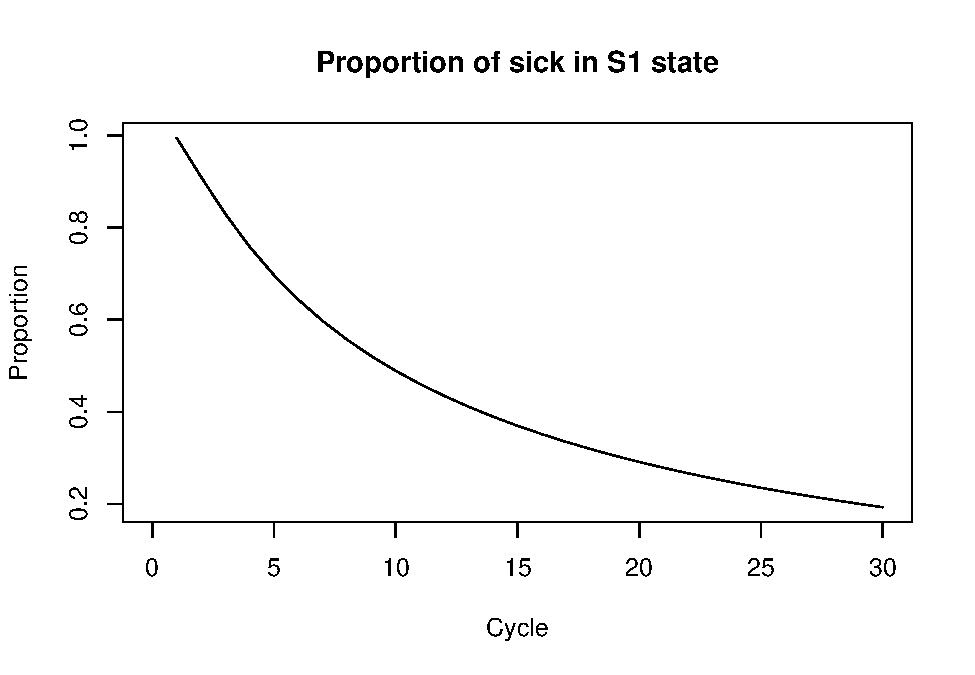
\includegraphics{Markov_3state_files/figure-latex/unnamed-chunk-13-1.pdf}

\hypertarget{compute-cost-effectiveness-outcomes}{%
\section{07 Compute Cost-Effectiveness
Outcomes}\label{compute-cost-effectiveness-outcomes}}

\hypertarget{mean-costs-and-qalys}{%
\subsection{07.1 Mean Costs and QALYs}\label{mean-costs-and-qalys}}

\begin{Shaded}
\begin{Highlighting}[]
\CommentTok{# per cycle}
\CommentTok{# calculate expected costs by multiplying m_M with the cost vector for the different }
\CommentTok{# health states   }
\NormalTok{v_tc <-}\StringTok{ }\NormalTok{m_M }\OperatorTok\StringTok{ }\KeywordTok{c}\NormalTok{(c_H, c_S, c_D)  }
\CommentTok{# calculate expected QALYs by multiplying m_M with the utilities for the different }
\CommentTok{# health states   }
\NormalTok{v_tu <-}\StringTok{ }\NormalTok{m_M }\OperatorTok\StringTok{ }\KeywordTok{c}\NormalTok{(u_H, u_S, u_D)  }
\end{Highlighting}
\end{Shaded}

\hypertarget{discounted-mean-costs-and-qalys}{%
\subsection{07.2 Discounted Mean Costs and
QALYs}\label{discounted-mean-costs-and-qalys}}

\begin{Shaded}
\begin{Highlighting}[]
\CommentTok{# Discount costs by multiplying the cost vector with discount weights (v_dw) }
\NormalTok{v_tc_d <-}\StringTok{  }\KeywordTok{t}\NormalTok{(v_tc) }\OperatorTok\StringTok{ }\NormalTok{v_dwc}
\CommentTok{# Discount QALYS by multiplying the QALYs vector with discount weights (v_dw)}
\NormalTok{v_te_d <-}\StringTok{  }\KeywordTok{t}\NormalTok{(v_tu) }\OperatorTok\StringTok{ }\NormalTok{v_dwe}
\end{Highlighting}
\end{Shaded}

\hypertarget{results}{%
\subsection{07.3 Results}\label{results}}

\begin{Shaded}
\begin{Highlighting}[]
\NormalTok{results <-}\StringTok{ }\KeywordTok{data.frame}\NormalTok{( }\StringTok{"Total Discounted Cost"}\NormalTok{ =}\StringTok{ }\NormalTok{v_tc_d, }
                       \StringTok{"Life Expectancy"}\NormalTok{ =}\StringTok{ }\NormalTok{v_le, }
                       \StringTok{"Total Discounted QALYs"}\NormalTok{ =}\StringTok{ }\NormalTok{v_te_d, }
                       \DataTypeTok{check.names =}\NormalTok{ F)}
\NormalTok{results}
\end{Highlighting}
\end{Shaded}

\begin{verbatim}
##   Total Discounted Cost Life Expectancy Total Discounted QALYs
## 1              8043.131        21.00019               10.18939
\end{verbatim}

\end{document}
